\documentclass[a4paper,12pt]{article}

\usepackage{amsmath,amssymb,amsthm,multicol,tikz,enumitem}
\usepackage{hyperref}
\usepackage{fancyvrb}
\usepackage[margin=2cm]{geometry}
\usetikzlibrary{calc,arrows.meta}

\newcommand\N{\mathbf{N}}
\newcommand\Q{\mathbf{Q}}
\newcommand\R{\mathbf{R}}
\newcommand\Z{\mathbf{Z}}

\def\ojoin{\setbox0=\hbox{$\bowtie$}%
  \rule[-.02ex]{.25em}{.4pt}\llap{\rule[\ht0]{.25em}{.4pt}}}
\def\leftouterjoin{\mathbin{\ojoin\mkern-5.8mu\bowtie}}
\def\rightouterjoin{\mathbin{\bowtie\mkern-5.8mu\ojoin}}
\def\fullouterjoin{\mathbin{\ojoin\mkern-5.8mu\bowtie\mkern-5.8mu\ojoin}}

\pagestyle{empty}


%\newcommand\answer[1]{}
%\newcommand\ans[1]{}
\newcommand\answer[1]{\\[5pt]{\color{blue}{#1}}\hfill{\color{blue}$\qed$}\\[-5pt]}
\newcommand\ans[1]{{\color{blue}{#1}}}


\newcommand\rem{\textup{rem}}

\begin{document}

\begin{center}
\parbox{3cm}{\flushleft\bf Discrete\linebreak Structures}
\hfill
\parbox{7cm}{\centering {\bf\Huge Exam, Part 2}}
\hfill
\parbox{3cm}{\flushright\bf Spring 2021 \linebreak May 27}
\end{center}

\hrule\vspace{2pt}\hrule

\hrule


\vspace{5pt}
\begin{enumerate}
\item
% 1.(c)
% Find members of arithmetic progressions, also by modulo m.
Let $a_n$ be an arithmetic series defined recursively:
\[ \left\{ \begin{array}{l}
a_0 = 0,\\
a_{n+1} = a_n + 19,\;\mbox{for $n \geq 0$}.\\
\end{array} \right. \]
\begin{enumerate}
\item How many members of this series $a_n$ are 3-digit numbers
(between $100$ and $999$)?
\answer{

{\bf Answer:} $47$.

All members of this series are divisible by $19$.
The smallest member $a_n$ that is at least $100$ (and is divisible by $19$)
is $a_6 = 6 \cdot 19 = 114$.

The largest member $a_n$ that does not exceed $999$ is
$a_{52} = 52 \cdot 19 = 988$.

The total number of such members
is $52 -6 + 1 = 47$. (We add $1$, because both members $a_{52}$ and $a_6$
should be included in the count.)

{\em Note.} We can do common-sense check for this answer.
In general, there are  $999 - 100 + 1 = 900$ numbers
having exactly three digits, and  $900/19 = 47.36842$.
So, among arithmetic series with common difference $d = 19$
some will have $47$ members in the interval $[100;999]$,
and some will have $48$ members in this interval.
In our case the sequence has $47$ members in the interval $[100; 999]$
}
\item What is the smallest member $a_k$ that satisfies
the congruence
$a_k \equiv 1 \pmod{16}$.
\answer{

{\bf Answer:} That member is $a_{11} = 11 \cdot 19 = 208$.

There are different ways to get this answer.

\vspace{5pt}
{\bf Method 1.} Observe that $19$ and $16$ are relative primes
($\text{gcd}(19,16) = 1$).
We solve the Bezout identity: Find integers $x,y$ satisfying the equation
\[ 19x + 16y = 1 \]
(You can apply Blankenship's algorithm or type this equation into Wolfram Alpha
or a similar tool. You will get $x = 11$ and $y = -13$, so $11 \cdot 19 + (-13) \cdot 16 = 1$.
We conclude that $a_{11} \equiv 1$ (modulo $19$).


{\bf Method 2.} In this problem we are interested into remainders modulo $16$.
So, we just need to find the multiplicative inverse of $19 \equiv 3$ (modulo $16$).
Observe that $3 \cdot 11 \equiv 33 \equiv 1 \pmod{16}$.
}
\end{enumerate}



\item
% 1.(d)
% Given two integers, find their GCD (also LCM) by Euclidean algorithm.
Consider the following two 5-digit numbers $a = 18696$ and $b = 99999$.
\begin{enumerate}
\item
Apply Euclidean algorithm to find the greatest common divisor $\text{gcd}(18696, 99999)$; show the steps of this algorithm.
Also find $\text{lcm}(18696, 99999)$.
\answer{

We start by dividing $99999$ with $18696$ (we get remainder $6519$). Then we replace
the largest number $99999$ with this remainder, and so on. This is the Euclidean algorithm.
\[ \gcd(99999,18696) = \gcd(99999,18696) = \gcd(18696, 6519) = \gcd(6519, 5658) = \]
\[ = \gcd(5658, 861) = \gcd(861, 492) = \gcd(492, 369) = \gcd(369, 123) = \gcd(123,0) = 123. \]

The least common multiple can be found by the formula $lcm(a,b) = ab/gcd(a,b)$:
\[ \text{lcm}(99999,18696) = \frac{99999 \cdot 18696}{\gcd(99999,18696)} = \]
\[ = \frac{99999 \cdot 18696}{123} = \frac{99999}{123} \cdot 18696 = 813 \cdot 18696 =  15199848. \]
}

\item
Express $\frac{18696}{99999}$ as an irreducible fraction.
\answer{

We can divide the numerator and denominator with their GCD:
\[ \frac{18696}{99999} = \frac{18696/123}{99999/123} = \frac{152}{813}. \]

{\em Note.} If we divide both numbers as an infinite decimal fraction, we will get
the same 5 digits (used in the problem statement) as the period:
\[ \frac{152}{813} = 0.186961869618696\ldots = 0.(18696). \]
}
\end{enumerate}



\item
% 1.(h)
% Given a decimal integer, convert it to binary, hexadecimal (and vice versa).
\begin{enumerate}
\item Let $\mathtt{1101011110}_2$ be a positive integer written in binary notation.
Convert this number into hexadecimal and also into decimal notation.
\answer{

Hexadecimal notation is easy \textendash{} just group the binary digits
into groups of $4$ (from the right side). You will get this:
\[  \mathtt{1101011110}_2 = \mathtt{11.0101.1110}_2 = \mathtt{35E}_{16}. \]

Decimal notation can be obtained either from the binary notation directly
(or from our hexadecimal notation). In the latter case we get:
\[ \mathtt{35E}_{16} = 3 \cdot 16^2 + 5 \cdot 16 + 14 = 862. \]

}
\item
Let $P(x)$ be polynomial with coefficients same as in this binary number (namely, $1, 1, 0, 1, 0, 1, 1, 1, 1, 0$):
\[ P(x)  = 1\cdot x^9 + 1\cdot x^8 + 0\cdot x^7 + 1\cdot x^6 + 0\cdot x^5 + 1\cdot x^4 + 1\cdot x^3 + 1\cdot x^2 + 1\cdot x^1 + 0\cdot x^0. \]
Evaluate this polynomial for $x=2$, i.e.\ find $P(2)$.
\answer{

You can simply note that the polynomial for $x=2$ evaluates to the numeric value of the
binary number $\mathtt{1101011110}_2$. So it must be $862$.

You can also compute this directly on a calculator. Figure~\ref{fig:part2-horner-scheme} shows
the screenshot from RStudio that computes $P(2)$:
\begin{figure}[!htb]
\center{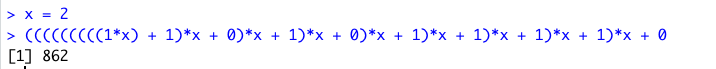
\includegraphics[width=4in]{figs/part2-horner-scheme.png}}
\caption{\label{fig:part2-horner-scheme} Evaluating Polynomial $P(x)$.}
\end{figure}
}
\end{enumerate}

\item
% 2.(a)
% Count the number of graphs with a given property or parameter.
Count the number of graphs having exactly $4$ vertices and
exactly $4$ edges.
All vertices in the graph are distinguishable, they are labeled with letters $A,B,C,D$,
and isomorphic graphs are considered different, if their vertex labels differ.
\answer{

Altogether there are $6$ edges you can draw between $4$ vertices in an undirected graph.
It will be easier for us to count the $2$ edges in the graph's complement (i.e.\ the two
not-taken edges in the graph) rather than $4$ edges that actually belong to the graph.

{\bf Case 1.} We can count those cases when the $2$ (non-existent) edges
share one vertex. In this case we would get a 'snake' or a 'path' of $3$ vertices connected
with edges.
For example, edges $\{ AB, BC\}$ create a short path $ABC$ with endpoints $A$ and $C$ and
$B$ in the middle.
Altogether there are $12$ ways to arrange three vertices on a  path.
\[ ABC, ABD, ACB, ACD, ADB, ADC, BAC, BAD, BCD, BDC, CAD, CBD. \]
In all these $12$ paths the first vertex alphabetically precedes the last one.
(There are $12$ more paths where the first vertex is alphabetically after the last one, but
they can be reversed so as to match one of the $12$ cases above.)

{\bf Case 2.} We can also count the cases where the $2$ (non-existent) edges
do not share any vertices. And there are just $3$ ways to
connect $4$ vertices with disconnected edges: $\{AB, CD\}$, $\{AC, BD\}$, and $\{AD, BC\}$.

Altogether there are $12 + 3 = 15$ ways to {\bf unselect} two vertices (and the same number of ways
to {\bf select} four vertices).
}

\item
% 2.(c)
% Convert between graph representations. Check if a graph is bipartite, complete, or connected.
An undirected graph $G=(V,E)$, where the vertices $V = \{ 0,1,2,3,4,5 \}$ is given by the following matrix:
\[ M_G = \left(
\begin{array}{cccccc}
0 & 1 & 1 & 1 & 1 & 0 \\
1 & 0 & 0 & 1 & 1 & 1 \\
1 & 0 & 0 & 0 & 1 & 0 \\
1 & 1 & 0 & 0 & 1 & 1 \\
1 & 1 & 1 & 1 & 0 & 0 \\
0 & 1 & 0 & 1 & 0 & 0 \\
\end{array}
\right) \]
\begin{enumerate}
\item Draw the representation of this graph as adjacency lists.
\item Find a Eulerian circuit in this graph: list its vertices or prove that it cannot exist.
\answer{

Eulerian circuit (a path that uses every edge exactly once and returns
to the starting point) in this graph exists.
This follows from the graph being connected and every vertex there has even degree \textendash{}
every row in the matrix has even number of 1s). The order of visiting vertices is
shown with the following path (it starts and ends in the vertex $(0)$):

\[ (0) \rightarrow (1) \rightarrow (3) \rightarrow (4) \rightarrow (0) \rightarrow (2) \rightarrow (4)
\rightarrow (1) \rightarrow (5) \rightarrow (3) \rightarrow (0). \]


\begin{figure}[!htb]
\center{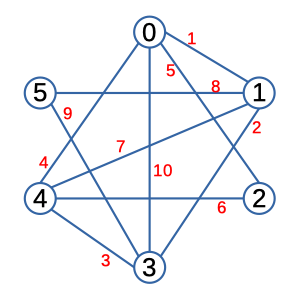
\includegraphics[width=2in]{figs/part2-eulerian-circuit.png}}
\caption{\label{fig:part2-eulerian-circuit} Graph with Eulerian circuit (edge order enumerated in red)}
\end{figure}

Figure~\ref{fig:part2-eulerian-circuit} shows this
circuit in the graph itself.
}
\end{enumerate}



\item
% 2.(c)
% Convert between graph representations. Check if a graph is bipartite, complete, or connected.
Let $G$ be a bipartite graph; all edges in this graph
connect some vertex in $V_1 = \{v_1, v_2, v_3, v_4 \}$ with some vertex in $V_2 = \{ v_5, v_6, v_7 \}$.
By $d(v_i)$ we denote the degree of some vertex.
\begin{enumerate}
\item Does there exist a bipartite graph  $G$ with these vertex sets, if the degrees of all $7$ vertices are as follows:
\[ (d(v_1), d(v_2), d(v_3), d(v_4), d(v_5), d(v_6), d(v_7)) = (2, 2, 1, 1, 2, 2, 1). \]
\answer{

This graph is impossible, since $2 + 2 + 1 + 1$ (sum of degrees on the left side of the bipartite graph)
is not equal to $2+2 + 1$ (the sum of degrees on the right side of the bipartite graph).
}
\item Does there  exist  a bipartite graph $G$ with these vertex sets, if the degrees of all $7$ vertices are as follows:
\[ (d(v_1), d(v_2), d(v_3), d(v_4), d(v_5), d(v_6), d(v_7)) = (3, 3, 1, 2, 3, 3, 3). \]
\answer{


\begin{figure}[!htb]
\center{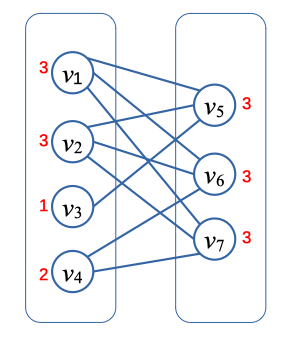
\includegraphics[width=1.5in]{figs/part2-bipartite-example.png}}
\caption{\label{fig:part2-bipartite-example} Example of a bipartite graph.)}
\end{figure}

Yes, such a graph exists (the sum of degrees are equal on both sides: $3+3+1+2 = 3+3+3$, and
no degree exceeds the number of vertices on the other side that it can connect with).
Figure~\ref{fig:part2-bipartite-example}
}
\end{enumerate}
{\em Note.} For each example draw some bipartite graph with these degrees (or explain why it cannot exist).

\end{enumerate}

\end{document}
